\documentclass{article} % For LaTeX2e
\usepackage{nips14submit_e,times}
\usepackage{hyperref}
\usepackage{url}
\usepackage{graphicx}
%\documentstyle[nips14submit_09,times,art10]{article} % For LaTeX 2.09


\title{Music Genre Classification Using Convolutional Neural Networks}


\author{
George Danforth \\
\texttt{gdanfor1@jhu.edu}
\And\-Edward Li \\
\texttt{eli8@jhu.edu}
}

\date{May 17, 2017}

% The \author macro works with any number of authors. There are two commands
% used to separate the names and addresses of multiple authors: \And and \AND.
%
% Using \And between authors leaves it to \LaTeX{} to determine where to break
% the lines. Using \AND forces a linebreak at that point. So, if \LaTeX{}
% puts 3 of 4 authors names on the first line, and the last on the second
% line, try using \AND instead of \And before the third author name.

\newcommand{\fix}{\marginpar{FIX}}
\newcommand{\new}{\marginpar{NEW}}

\nipsfinalcopy% Uncomment for camera-ready version

\begin{document}


\maketitle

\begin{abstract}
TODO
\end{abstract}

\section{Introduction}
The task of automatically classifying pieces of music by genre has various applications; from helping people discover music they like more quickly and easily, to investigating and understanding the differences between musical genres in an empirical fashion. In spite of the potential applications, this task is also a particularly difficult one\ldots TODO


\section{Related Work}
\subsection{Audio Feature Extraction}
The foundation of performing any kind of automatic audio analysis is the ability to retreive descriptive features from an audio signal. Although many different methods of audio feature extraction have been proposed for various applications, some of the most widely employed features for the task of audio classification are mel-frequency cepstral coefficients (MFCCs), and pitch histograms~\cite{survey}. MFCCs~\cite{mfcc} are perceptually motivated features which, at a high level, can be said to describe the timbre of an audio signal over time, and are computed on individual frames of a signal by applying various transformations to their power spectra. Pitch histograms are a way of measuring the representation of discrete pitches (usually on a 12-tone scale) at different time frames throughout and audio signal~\cite{gtzan}.

\subsection{The Million Song Dataset}
The Million Song Dataset (MSD) is a collection of metadata and audio features over one million pieces of music spanning a variety of genres and time periods. In a collaboration between The Echo Nest and the Columbia University Laboratory for the Recognition and Organization of Speech and Audio (LabROSA), the MSD has been made freely available to the public with the goal of encouraging research into applying machine learning methods to musical data~\cite{msd}.
\par The metadata features included in the MSD consist of basic information such as the artist of the track, the year it was released, the album or compilation it was released on, etc. Additionally, each track contains a list of tags relating to the artist, which have been compiled by the MusicBrainz community.
\par Each track in the MSD also contains numerous audio features, both at the track level and corresponding to individual segments within a track, which have been extracted by The Echo Nest. The track level features include tempo, time signature, and key, as well higher level features created by The Echo Nest, such as ``danceability'', and ``energy''. For more fine-grained information, each track in the MSD was broken up into a number of variable time-length segments, each roughly corresponding to a note/bar onset or some other relevant musical event. The features included at the segment level include length-12 vectors of timbre features, which are described as MFCC-like features, length-12 vectors of pitch information, which are normalized pitch histograms, as well as the maximum loudness within each segment.


\subsection{Other Models}


\section{Method}
\subsection{Data Reduction and Preprocessing}
Despite the wealth of information and features provided by the MSD, there was still a significant amout of work to do to reduce the data into a format suitable for our classification task. One of the major setbacks of using the MSD for this classification task is that it does not come with genre labels for each track. As a work-around, we compiled the most common MusicBrainz tags across the entire dataset, and manually selected the most common genres out of them, as well as tags and genre variants that appeared most often together with these genres. We then went back through the dataset and computed a score for each track based on the degree to which its tags intersected with the tags for each genre, and selected a genre based on this score. Any tracks lacking MusicBrainz tags completely were not included in the training or evaluation sets.
\par As part of the data reduction we also had to decide what features to use. Since we were interested in using low-level audio features only, and we intended to use a convolutional neural network to compare features at different time scales, we chose to use only segment-level features. Namely, for each segment we used the timbre vector, and the pitch histogram vector, and the maximum loudness. Since each track consisted of a variable number of segments, ranging from one into the thousands, we computed the minimum number of segments such that 95\% of the data points would have a greater number of segments. Finding this value to be roughly 120, we chose the central 120 segments of each track having greater than or equal to 120 segments, and constructed our training and validation sets such that each data point had 3000 features: $120 \times (1 + 2 \times 12)$. As a final preprocessing step, we subracted the per-feature mean and divided by the per-feature standard deviation across the entire reduced dataset.

\subsection{Convolutional Layer Implementation}
Instead of treating each data sample as a set of 3000 individual features as we do under a regular (fully-connected) neural network, we can treat it as 120 slices of a time dimension with 25 unique acoustic features each. Since certain musical patterns of songs may last longer than others, we may wish to study the patterns these 25 features exhibit over different regions of time. This makes our dataset a good candidate for study under a convolutional neural network.

Unlike a regular neural network where neurons are arranged in single-dimensional layers, in a convolutional neural network, neurons are arranged in two-dimensional layers: the ``length'' dimension corresponds to a region of time within the song and the ``depth'' dimension corresponds to a ``filter''. Each filter is just a set of weights and a bias which are applied to a region of time smaller than the total output region passed by the previous layer. Each layer of the neural network may have multiple filters, all of which are of the same length and are unique to that layer.

In some sense, we can treat each individual filter as a fully-connected layer: a filter's forward for a single region of time acted on by that filter is the same as the forward pass of a full-connected layer. Hence, for a filter $i=\{1,2,\ldots,n^{(l)}\}$ in layer $l$ with weight $W^{(l)}_i$, bias $b^{(l)}_i$, and input $Z^{(l)}_{ij}$, we have
\begin{equation}
    z^{(l+1)}_{ij} = W^{(l)}_i Z^{(l)}_{ij} + b^{(l)}_i
\end{equation}
However, each filter in layer $l$ acts over the entire output passed by layer $l-1$. In our implementation, we use a stride of 1 since we only have 120 slices of time. Hence, if layer $l$ has a filter size of $a^{(l)}$ and layer $l-1$ produces an output length of $b^{(l-1)}$, then each filter input $Z^{(l)}_{ij}$ contains $a^{(l)}$ consecutive elements of the output from layer $l-1$ and $j=\{1,2,\ldots,b^{(l-1)}-a^{(l)}+1\}$. Therefore, layer $l+1$ contains $b^{(l-1)}-a^{(l)}+1$ elements in the length dimension and $n^{(l)}$ elements in the depth dimension.

Because of the behavior of each filter in a convolutional neural network layer, backpropagation here is handled a little differently from backpropagation in a fully-connected neural network layer. In our loss gradients for layer $l$, instead of having a contribution of loss to each of the neurons in layer $l+1$, we have a contribution of loss to each filter output, which corresponds to each depth element of layer $l+1$. Additionally, the contribution of loss to a depth element of layer $l+1$ from an input element of layer $l$ is summed over up to $n^{(l)}$ different derivatives with respect to the weight vectors contained in the set of weights for the corresponding filter of layer $l$. Of course, input elements near the ends of the time dimension have fewer derivatives with respect to the weight vectors since they contribute to fewer elements in the output region.


\section{Results}
\begin{figure}[h]
\centering
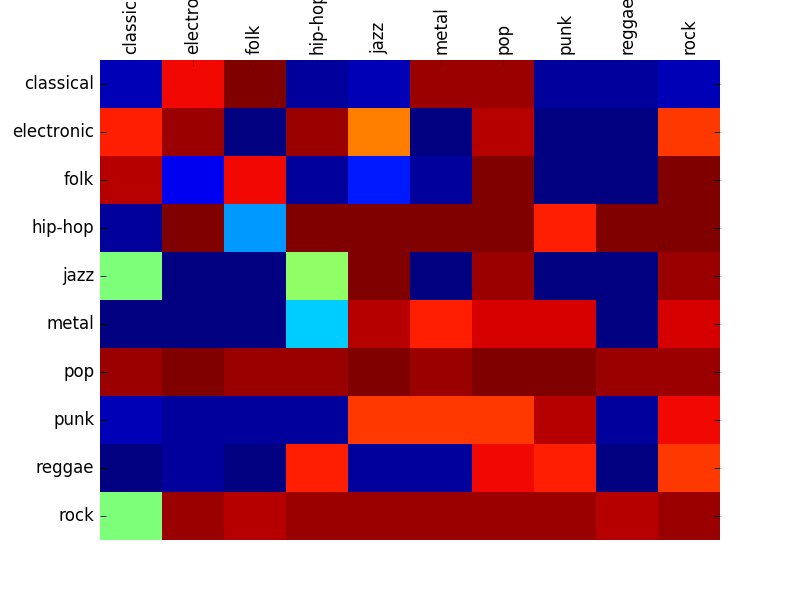
\includegraphics[scale=0.5]{confusion}
\end{figure}
\section{Conclusion}
\section{Discussion}
\section{Further Work}
\begin{thebibliography}{10}
\bibitem{survey}
Zhouyu Fu, Goujun Lu, Kai Ming Ting, Dengsheng Zhang.
\textit{A Survey of Audio-Based Music Classification and Annotation}.
IEEE Transactions on Multimedia, 2010.

\bibitem{mfcc}
S. Davis, P. Mermelstein.
\textit{Experiments in Syllable-Based Recognition of Continuous Speech}
IEEE Transactions on Acoustic, Speech, and Signal Processing, vol. 28, pp. 357--366, 1980.

\bibitem{msd}
Thierry Bertin-Mahieux, Danile P.W. Ellis, Brian Whitman, Paul Lamere.
\textit{The Million Song Dataset}.
Proceedings of the 12th International Society for Music Information Retrieval Conference (ISMIR 2011), 2011.

\bibitem{gtzan}
George Tzanetakis, Perry Cook.
\textit{Musical genre classification of audio signals}.
IEEE Transactions on Speech and Audio Processing, vol. 10, no. 5, pp. 293--302, 2002.
\end{thebibliography}

\end{document}
